\documentclass{../../../../style/mkimain}

\series{4}
\month{květen}
\year{2023}

\begin{document}
%<*header>
\section*{IV.U1 Header4-U1}
%</header>
%<*task>

\noindent K následujícím obrázkům přiřaďte jev, nebo objekt, který zachycuje.

\vspace{0.5cm}
\begin{mdframed}[frametitle={Díla}, frametitlealignment=\center, innerbottommargin=5px]
    \begin{center}
        speciální~princip~relativity, gravitační~zákon, elektromagnetická~indukce, stanovení~teploty~černé~díry, myšlenkový~experiment~s~kočkou~v~krabici, teorie~radioaktivity
    \end{center}
\end{mdframed}
\vspace{1cm}
\begin{figure}[H]
  \minipage{0,2\textwidth}
    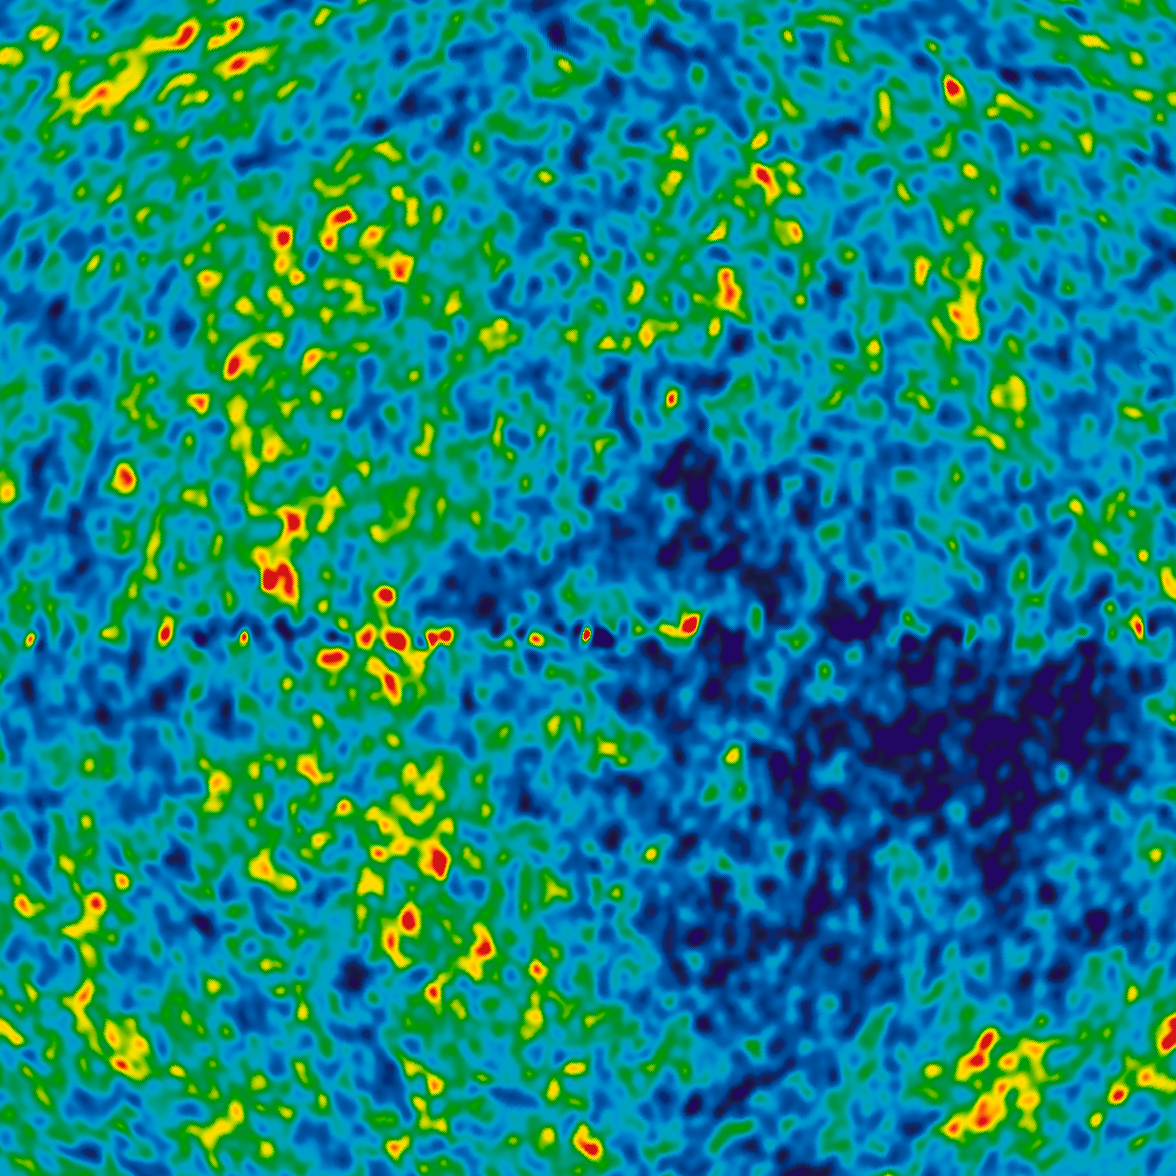
\includegraphics[width=\linewidth]{images/reliktni-zareni.png}
    \begin{center}
      1 Credit: NASA/WMAP Science Team
      \end{center}
  \endminipage\hfill
  \minipage{0.2\textwidth}
    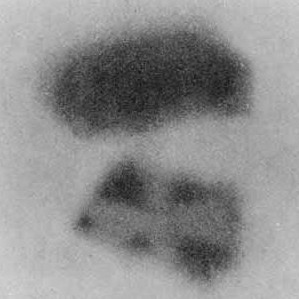
\includegraphics[width=\linewidth]{images/becquerel.jpg}
    \begin{center}
      2
      \end{center}
  \endminipage\hfill
  \minipage{0.2\textwidth}%
    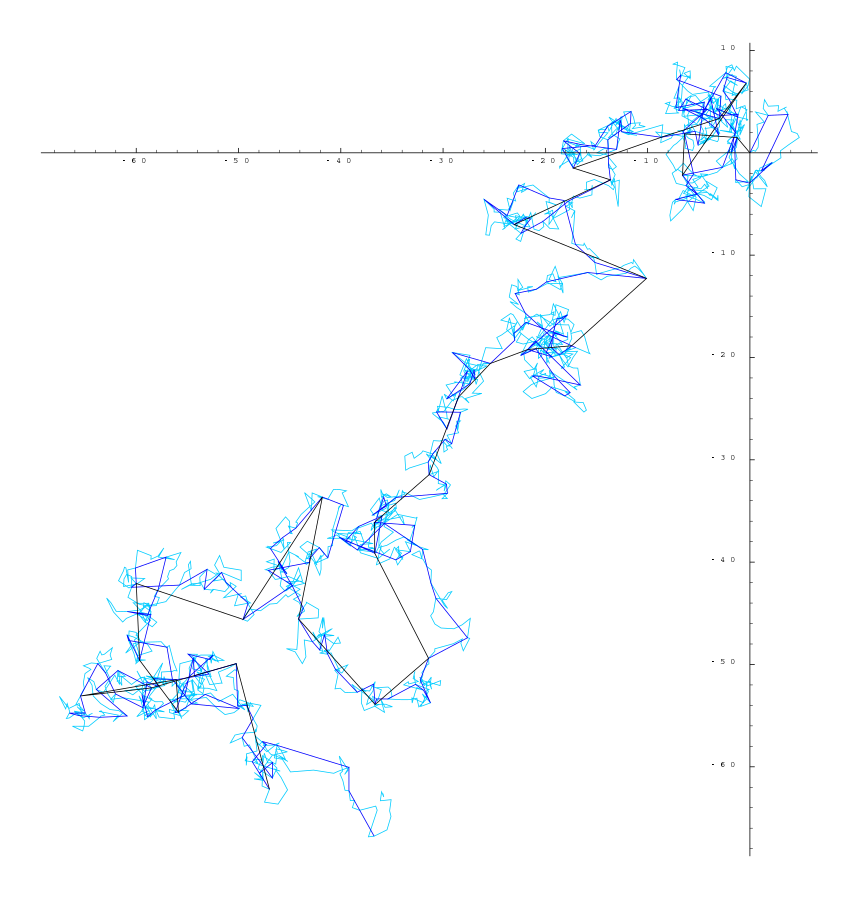
\includegraphics[width=\linewidth]{images/brownuv-pohyb.png}
    \begin{center}
    3
    \end{center}
  \endminipage
\end{figure}
\vspace{0.5cm}
\begin{figure}[H]
  \minipage{0.2\textwidth}
    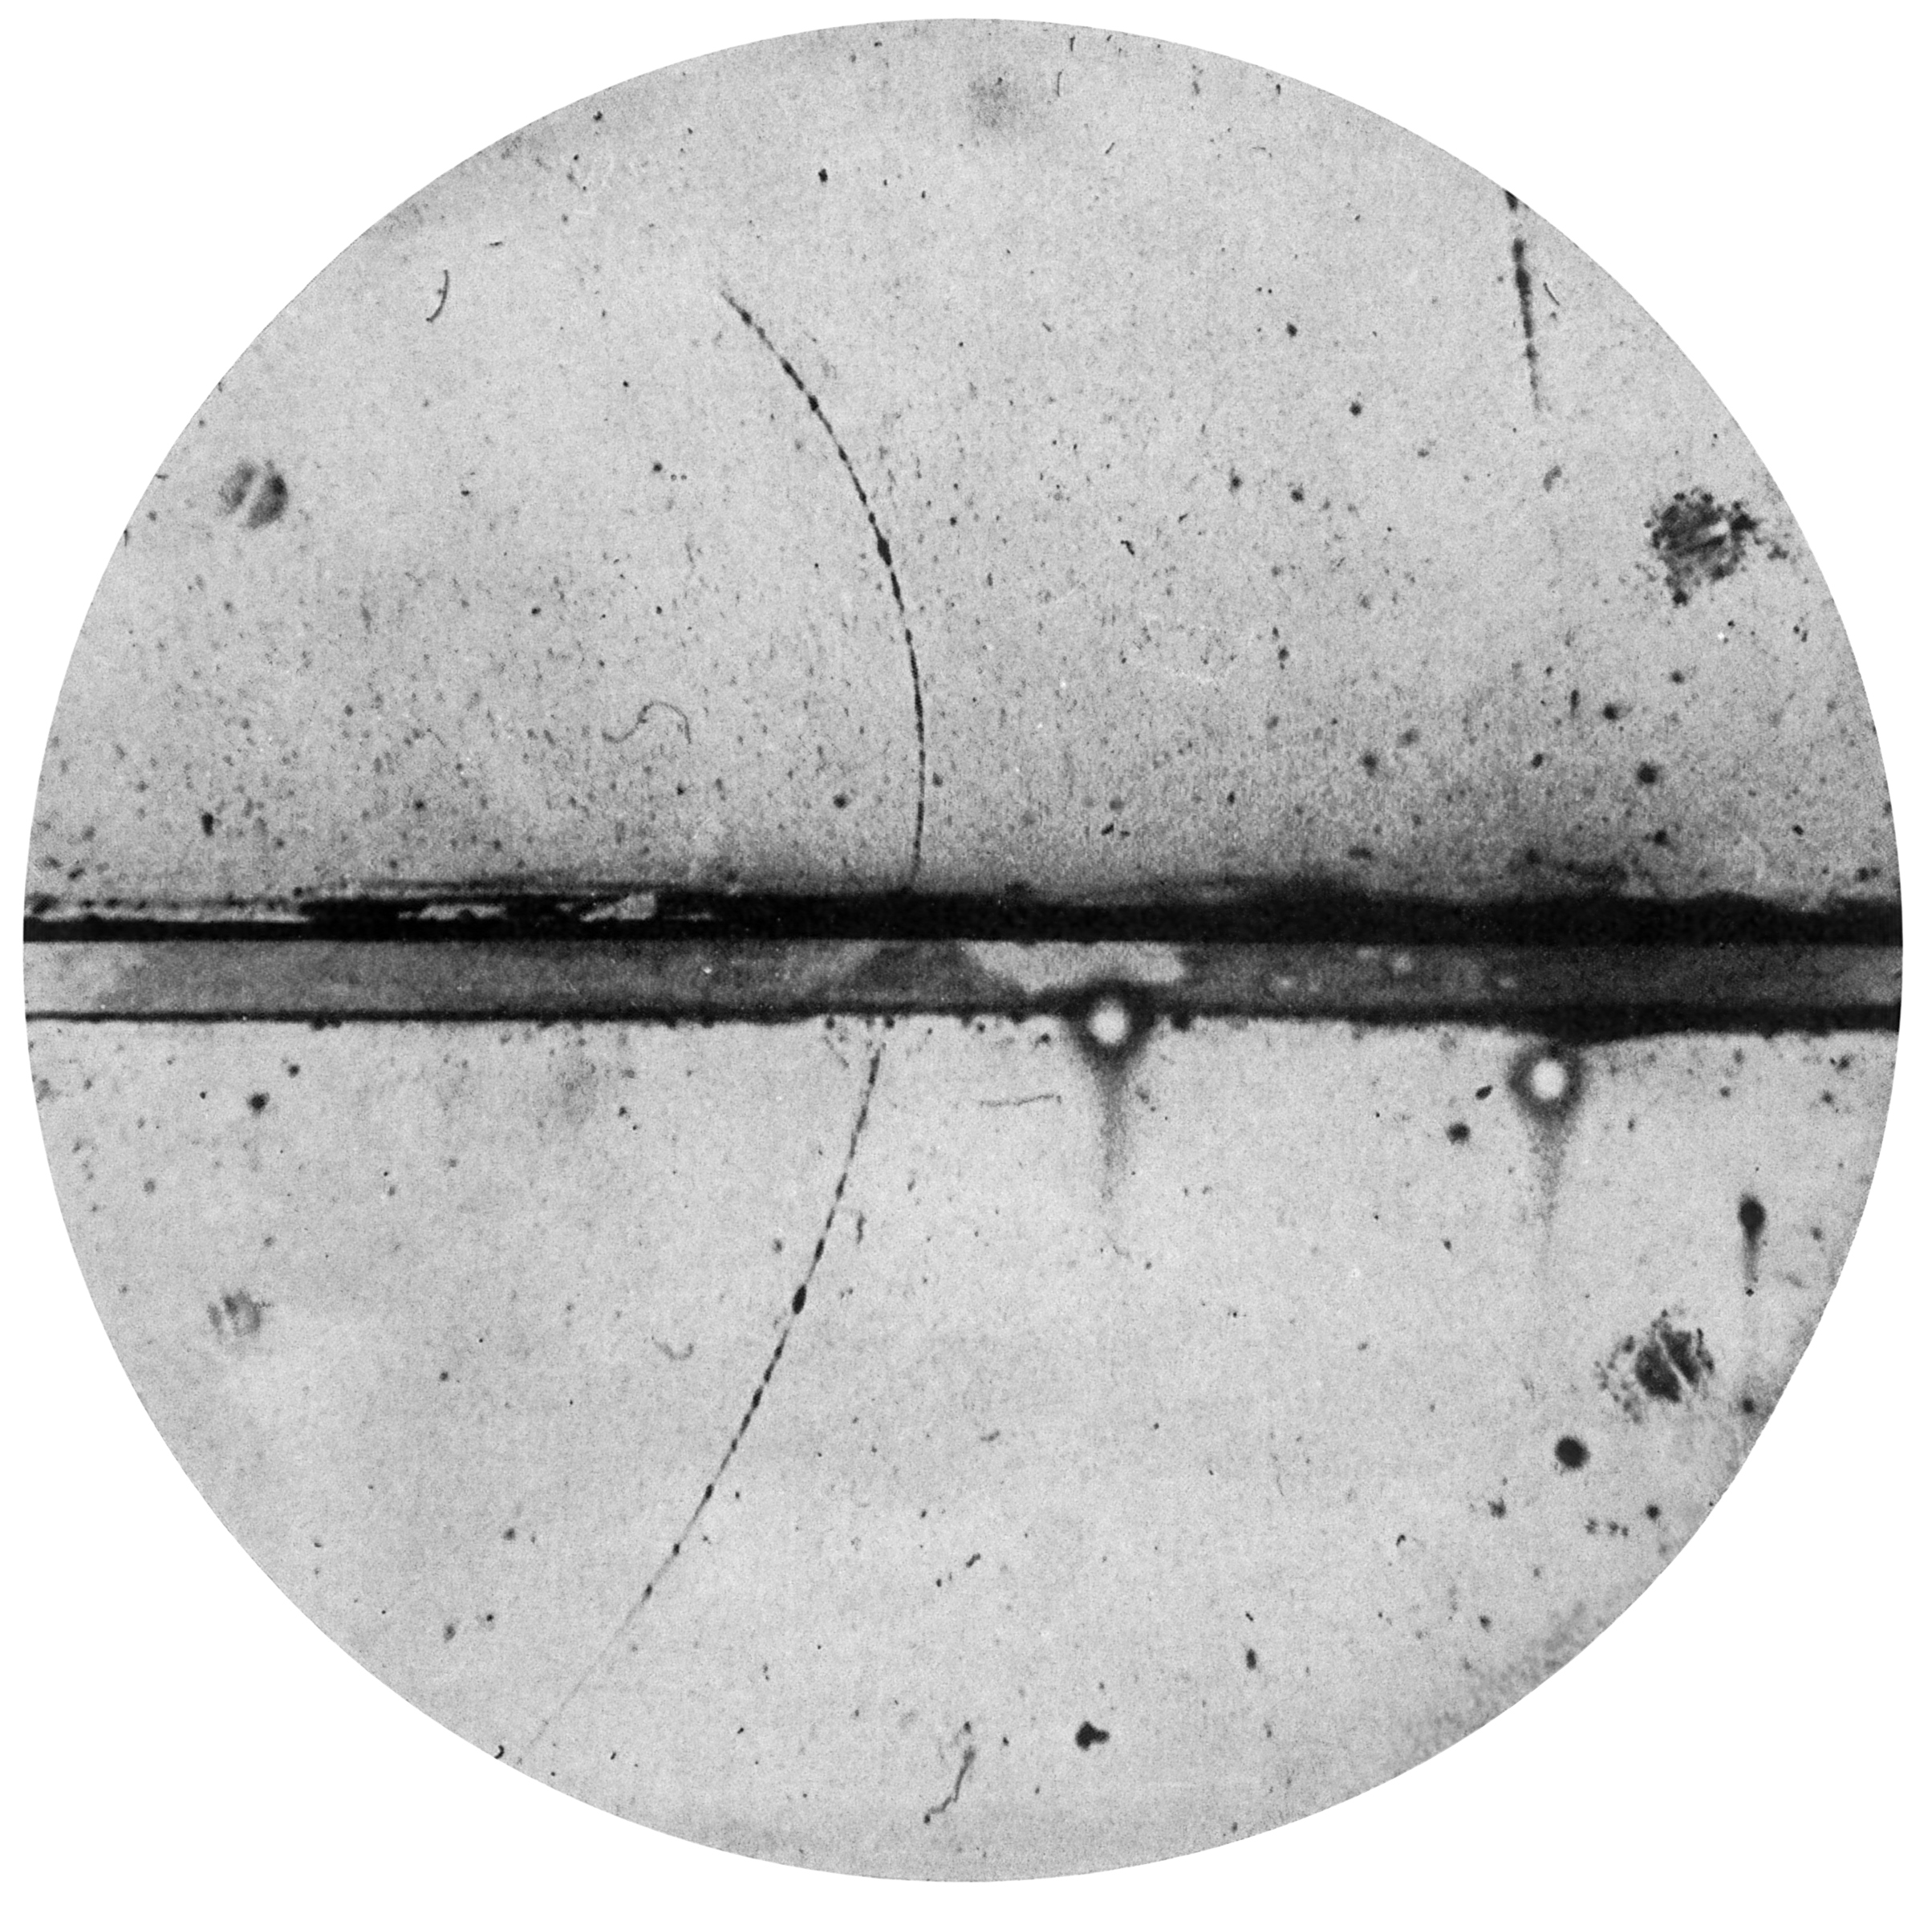
\includegraphics[width=\linewidth]{images/pozitron.jpg}
    \begin{center}
      4 EHT Collaboration
      \end{center}
  \endminipage\hfill
  \minipage{0.2\textwidth}
    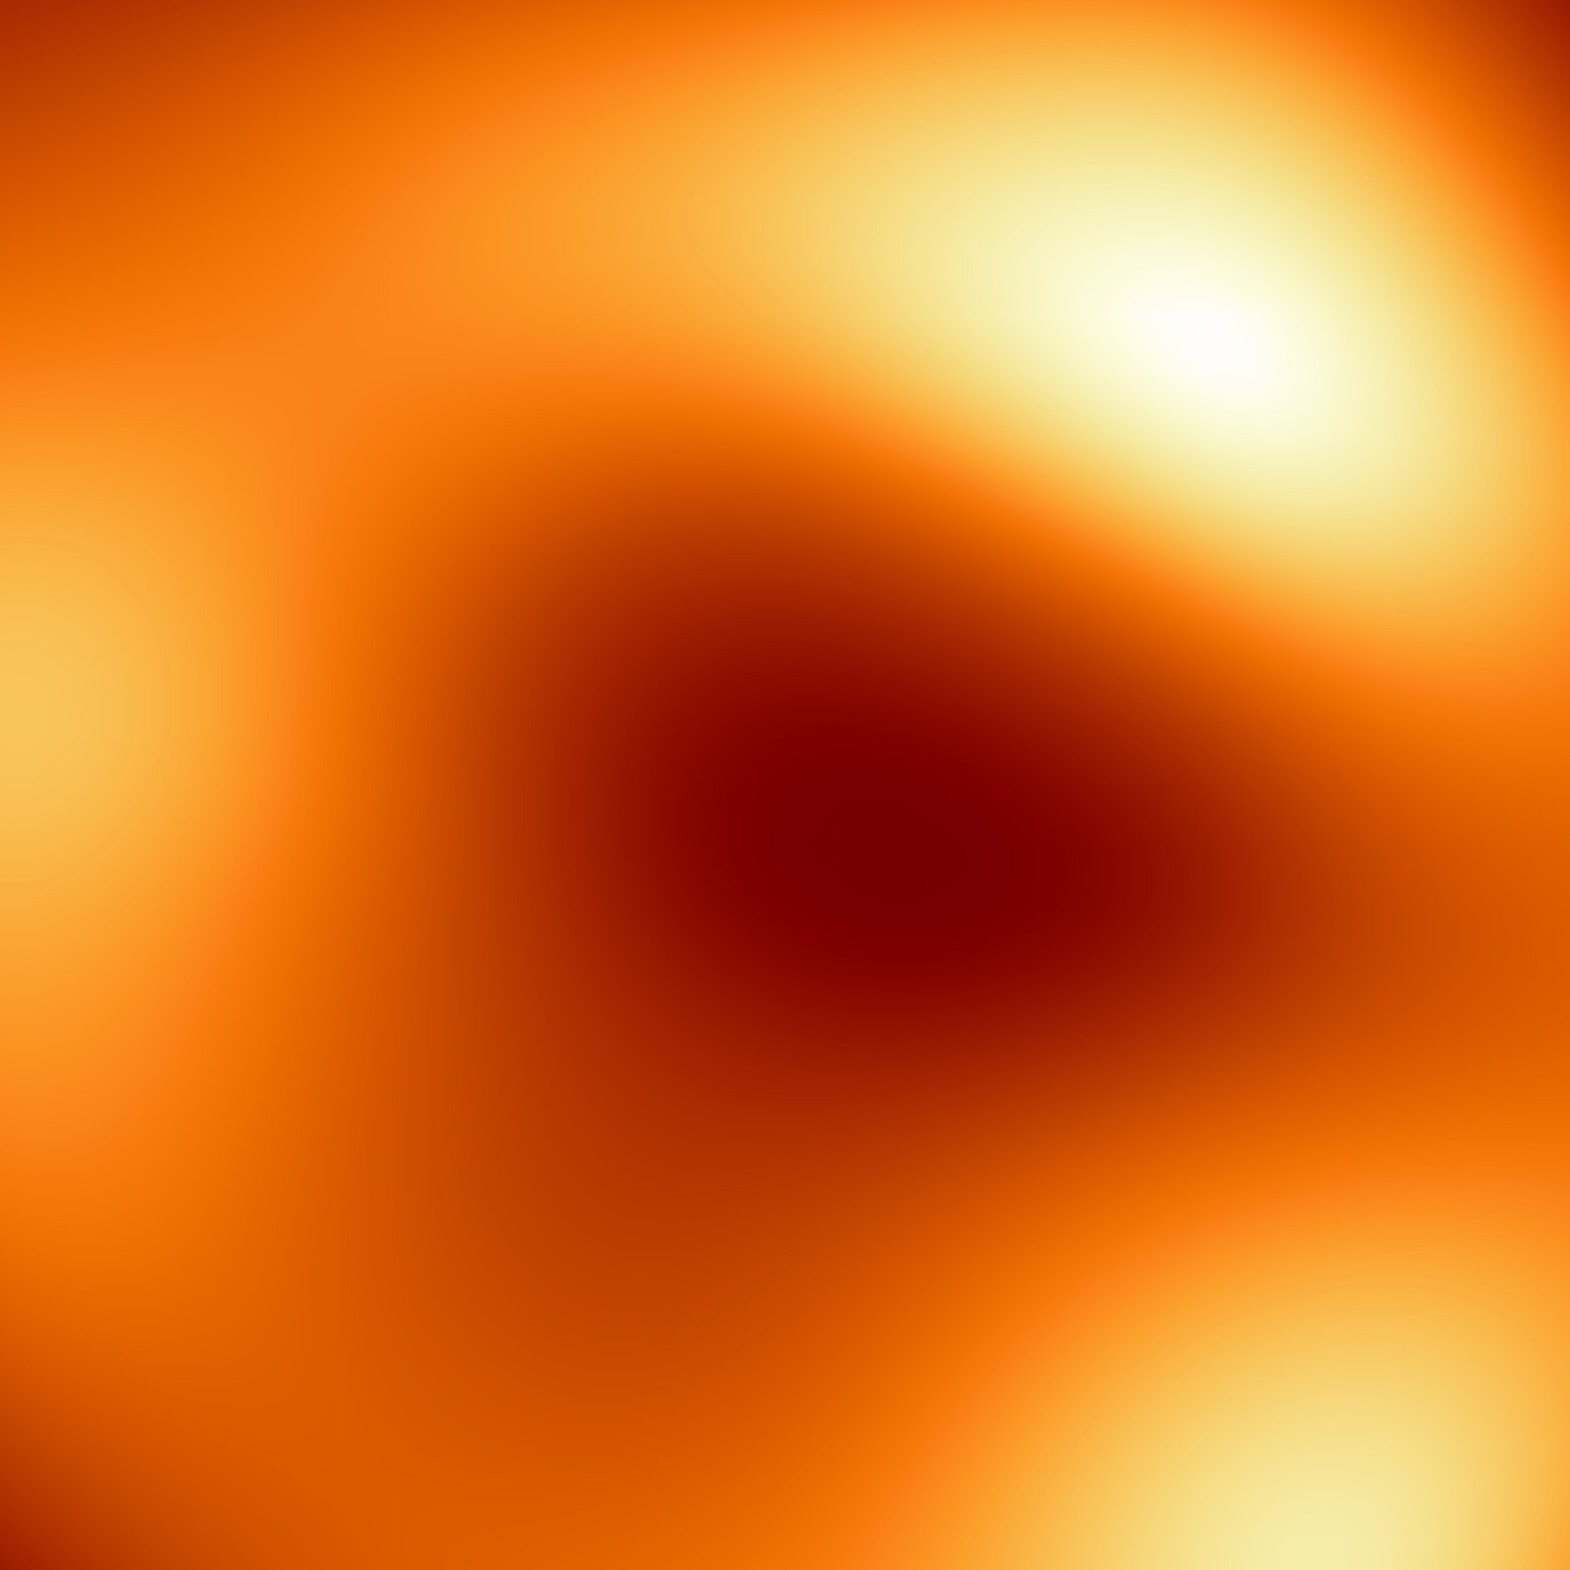
\includegraphics[width=\linewidth]{images/sagittarius.jpg}
    \begin{center}
      5 Creative Licensed under Commons Attribution-Share Alike 3.0 Unported <- link https://creativecommons.org/licenses/by-sa/3.0/deed.en
      \end{center}
  \endminipage\hfill
  \minipage{0.2\textwidth}%
    \includegraphics[width=\linewidth]{images/}
    \begin{center}
      6
      \end{center}
  \endminipage
\end{figure}

%</task>
\end{document}
